\section{FFS}
The artifact that was developed as a result of this thesis is the Fejk FileSystem (FFS). It uses an online web service (OWS) to store the data but behaved as a mountable filesystem for the users. The filesystem is a proof-of-concept and does not support all functionalities that other filesystems do, such as links or access permissions. The reasoning is that these behaviors are not required for a useable system, and when comparing the filesystem to distributed filesystems such as Google Drive, many of these other filesystems also often do not support functionality such as links.

\subsection{Design overview}
FFS uses images to store the data of files, directories and the inode table of the filesystem. These images will are uploaded to the OWS, such as Flickr, as image posts. As mentioned in Section~\ref{sec:ows}, there can be limitations to these posts for certain OWSs. To support file sizes bigger than these limitations, bigger files will be split into multiple posts, requiring FFS to keep track of a list of posts. Figure~\ref{fig:ffs_inode_diag} presents the basic outline of FFS and a example content of the filesystem. FFS is based on the idea of inode filesystems and uses a inode table to store information about the files and directories in the filesystem. However, instead of an inode pointing to specific blocks in a disk, the inode table of FFS will instead keep track of the id numbers of the posts on the OWS where the file or directory is located. The inode table entry for each file or directory will also contain metadata about the entry, such as its size and a boolean indicating if the entry is a directory or not.

\begin{figure}[!ht]
	\begin{center}
	  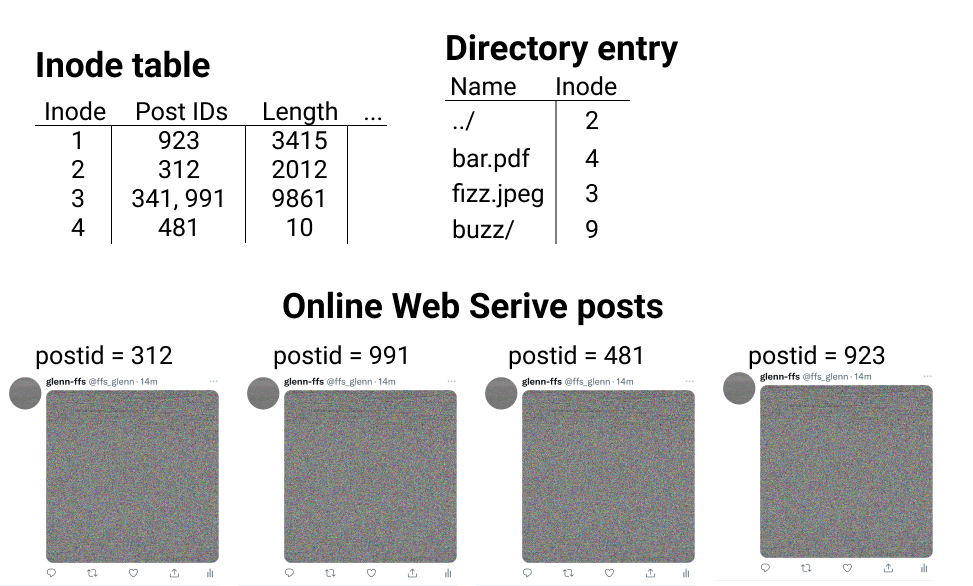
\includegraphics[width=0.8\textwidth]{figures/ffs_inode_diagram.png}
	\end{center}
	\caption{Basic structure of FFS inode-based structure}
	\label{fig:ffs_inode_diag}
\end{figure}

The directories and inode table are represented as classes in C++. Appendix~\ref{app:inode_dir_code} visualizes the main attributes of the \texttt{Directory}, \texttt{InodeTable}, and \texttt{InodeEntry} classes. There can be multiple \texttt{Directory} and \texttt{InodeEntry} objects in the computers' memory and in the filesystem, but there will only exist one \texttt{InodeTable} instance which is relevant. The \texttt{Directory} class is a data structure that stores mappings between filenames and the files' and directories' inode for all files and directories stored in that directory. The \texttt{InodeEntry} is a data structure that keeps track of a file's or directory's information, such as where the data is stored and its metadata, such as size and creation timestamp. The \texttt{InodeTable} stores a mapping between an inode and the files' \texttt{InodeEntry}, and stores all the \texttt{InodeEntry} objects. The \texttt{InodeTable} always has at least one entry which is the root directory. This entry has a constant inode value of 0 for simplicity to look up the root directory. With the help of the root directory, all the files lower in the directory hierarchy can be found. The inode of all files and directories other than the root directory has a unique inode greater than 0. The \texttt{InodeTable} is saved on the OWS through such means that it can easily be found, for instance by tagging the image post it with a unique string so it can be found by a search.

To read the content of a known file in a directory has three steps:
\begin{enumerate}
	\item The \texttt{Directory} object of the directory provides the inode of the given filename.
	\item The inode is used to get the \texttt{InodeEntry} from the \texttt{InodeTable}.
	\item Using the inode entry, the the file can be located.
\end{enumerate}
The location of a file or directory is an ordered list of unique IDs of the image posts on the OWS. The data received by downloading these images, decoding them (as described in Subsection~\ref{subsec:file_enc_dec}), and concatenating them, can be read as a file or represented as a \texttt{Directory} object, depending on if the \texttt{InodeEntry} was marked as a file or a directory. 

As directories only know the filenames inode, the \texttt{Directory} object does not have to be saved again (and thus uploaded) when a file or directory in it is edited, for instance adding data. Only the \texttt{InodeEntry}, and thus the \texttt{InodeTable}, needs to be updated with the new post IDs of the new file or directory. This saves computation time as every request to the OWS takes time. However, if the filename is edited or the file or directory is moved to another location, the parent directory of the file or directory would have to be edited, and such its corresponding \texttt{Directory} object has to be updated.

When a new file or directory is created, it is saved in its parent directory with its filename and an inode. The same inode is used in the inode table to keep track of the file's or directory's inode entry. As shown in Appendix~\ref{app:inode_dir_code}, the inode is represented as a unsigned 32-bit integer. The inode is calculated by adding one to the currently greatest inode. This means that new files and directories will always receive a higher greater inode than the ones currently in the inode table. This naïve approach to inode generation does not take in to account that there might be an available inode less than the greatest inode in the inode table (for instance, due to deletion of a previously created file). However, this inode generation approach is fast and will not be a problem until the integer overflows. As the inode is represented using a 32-bit integer, FFS would need to have saved over four billion files before the inode value would overflow. This scenario is not in the scope of this proof-of-concept filesystem.

FFS does not support all filesystem operations that are implementable through FUSE, instead FFS implements a subset of them. The implemented functions are shown in Table~\ref{tbl:fs_impl_op}. The implemented operations are the most vital operations required for a working filesystem\,\cite{kuenningCS135FUSEDocumentation2010}. Operations such as \texttt{chown} provides extended capabilities of the filesystem but these are not required for a proof-of-concept filesystem. The functionality of the filesystem operations implemented by FFS and their implementation details are described in Subsection~\ref{subsec:file_op}. 

\begin{table}[!ht]
	\begin{center}
		\caption{Filesystem operations implementable trough the FUSE API, and wether or not FFS implements them}
		\begin{tabular}{| c | c |}
			
			\hline
			\textbf{Filesystem operation} 	& \textbf{Implemented by FFS}\\
			\hline
			\hline
			\texttt{open} & Yes\\
			\texttt{opendir} & Yes\\
			\texttt{release} & Yes\\
			\texttt{releasedir} & Yes\\
			\texttt{create} & Yes\\
			\texttt{mkdir} & Yes\\
			\texttt{read} & Yes\\
			\texttt{readdir} & Yes\\
			\texttt{write} & Yes\\
			\texttt{rename} & Yes\\
			\texttt{truncate} & Yes\\
			\texttt{ftruncate} & Yes\\
			\texttt{unlink} & Yes\\
			\texttt{rmdir} & Yes\\
			\texttt{getattr} & Yes\\
			\texttt{fgetattr} & Yes\\
			\texttt{statfs} & Yes\\
			\texttt{access} & Yes\\
			\texttt{utimens} & Yes\\
			\texttt{readlink} & No\\
			\texttt{symlink} & No\\
			\texttt{link} & No\\
			\texttt{chmod} & No\\
			\texttt{chown} & No\\
			\texttt{fsync} & No\\
			\texttt{fsyncdir} & No\\
			\texttt{lock} & No\\
			\texttt{bmap} & No\\
			\texttt{setxattr} & No\\
			\texttt{getxattr} & No\\
			\texttt{listxatt} & No\\
			\texttt{ioctl} & No\\
			\texttt{flush} & No\\
			\texttt{poll} & No\\
			\hline

		\end{tabular}
		\label{tbl:fs_impl_op}
	\end{center}
\end{table}

A file, a directory, or the inode table has to be uploaded to the OWS when it is modified to save its current information. As it takes time to make requests to the OWS, FFS is created to make as few requests as possible while still saving the data required. Therefor, only the directory or file that is affected by a change is uploaded to the system, while the ones unaffected can remain the same. The inode table has to be updated with every change of a file or directory as it contains the location of the file or directory.

\subsection{Cache}
FFS implements a simple cache for the downloaded content. The cache consists of two data structures: 
\begin{itemize}
	\item a Cache Map - a mapping between a post ID and its image data, and
	\item a Cache Queue - a queue keeping track of the cached post IDs.
\end{itemize}
The cache stores a maximum of 20 image posts. To avoid FFS to use too much memory, the cache is configured so that images greater than \SI{5}{\mega\byte} are not cached. Each time an image is uploaded or downloaded, it is added to the Cache Map with its post ID as the key. The post ID is also added to the beginning of the Cache Queue. If the Cache Queue exeeds 20 elements, the last elements of the queue is removed, and the corresponding entry in the Cache Map is erased, thus the entry is fully erased from the cache. The queue ensures that the chache is limited to 20 entries, and by using the first in first out valuation method, the queue also ensures that the oldest element in the cache is removed when the cache exeeds the limit. When a file or directory is removed from the filesystem, all its data is also removed from the cache, if it stored there.

Before a post with a specified post ID is downloaded from the OWS, the cache is checked to see if it is storing this post ID. If it is, the stored image is returned. Otherwise, the process continues by downloading the image from the OWS. When the thesis states that a file or directory is downloaded, it is implied that the cache is also checked and the data is possibly returned by the cache instead of requiring to download the data from the OWS.

FFS separately caches both the root directory and the inode table. As both of these data structures are used in many of the filesystem operations, it is important that they can be accessed quickly and not be removed from the cache. Their cache entries are updated when the files are uploaded to the OWS.

\subsection{Encoding and decoding objects}
\label{subsec:file_enc_dec}
Objects that FFS stores, and therefore also encodes and decodes, are: files, directories, and the inode table. All of these objects are stored on the OWS using PNG images with 16 bit RGB color depth. The inode table and the directories are represented as C++ objects in memory during runtime, but are serialized into a binary representation before they are encoded into images. A detailed description of these binary formats is described in Appendix~\ref{app:binary_rep}. The files saved to FFS are also read in to memory in a binary format before being encoded and uploaded to the OWS. 

The input to the image encoder is the binary data do encode as an image. A header (FFS header) is prepended to the binary data, containing among other things, the size of the data and a timestamp of when the data was encoded. The FFS header and the input data is encrypted using authenticated encryption, utilizing GCM and AES. The key used for the encryption is derived using the HKDF function utilizing the SHA-256 hashing algorithm, along with a \SI{64}{\byte} salt vector, re-generated with random data every time new data is being encrypted. The salt is stored with the cipher to ensure that the decryption algorithm uses the same salt to derive the decryption key. The secret used in the HKDF is a password provided by the user. HKDF also uses a initialization vector, re-generated with random data every time new data is being encrypted. The length of the IV is set to 12 bytes. The resulting data from the encryption is the salt, the IV, the encrypted cipher (including the authentication tag). These three data points are concatenated into a string of bytes. This string of bytes is referred to as the Complete Encrypted Data (CED).

The dimensions of a FFS image is based on the amount of bytes stored, as described in Section~\ref{sec:data_storage}. The stored data is the CED, prepended with the length of the CED (LCED) using 4 bytes. For an image of $X = ceil(\frac{4 + LCED}{6})$ pixels, FFS will set the width $w$ of the image as $w = ceil(\sqrt{X})$. Further, the height $h$ of the image is set as $h = ceil(\frac{X}{w})$. This will require $(w * h) - X$ filler bytes, and will create an image with similar height and width. For certain values of $X$, $h$ will be equal to $w$. For other values of $X$, $h = w-1$. The resulting data encoded in the image is, in order:
\begin{itemize}
	\item 4 bytes representing the LCED,
	\item The CED data, and
	\item Filler bytes
\end{itemize}
The filler bytes are randomized bytes.

The data consisting of the LCED, CED and filler bytes is encoded in to pixel color data for a PNG with 16 RGB bit color depth using the Magick++ library. The result is an image, with a high probability, of what looks like randomized colors for each pixel. This is due to the fact that most pixels are encrypted and therefore the bytes representing this data is seemingly random.

To decode a FFS image, the decoder first interprets the 4 first bytes as the LCED. The following $LCED$ bytes are decrypted using the same key as mentioned above, as AES is a symmetric cipher algorithm. The unencrypted data consists of the FFS header concatenated with the original stored data. The header is asserted to be in the correct format, before the stored binary data is read and returned.  Figure~\ref{fig:file_enc_dec} visualizes the encoder and decoder for all data saved in FFS.

% TODO: Mention upper limit of FFS image size here
A FFS image has an upper size limit, defined by the OWS used. Further, an image storing data can become bigger than the data it stores. During testing of different filetypes and data sizes, this has been found to exceed 


\begin{figure}[!ht]
	\begin{center}
	  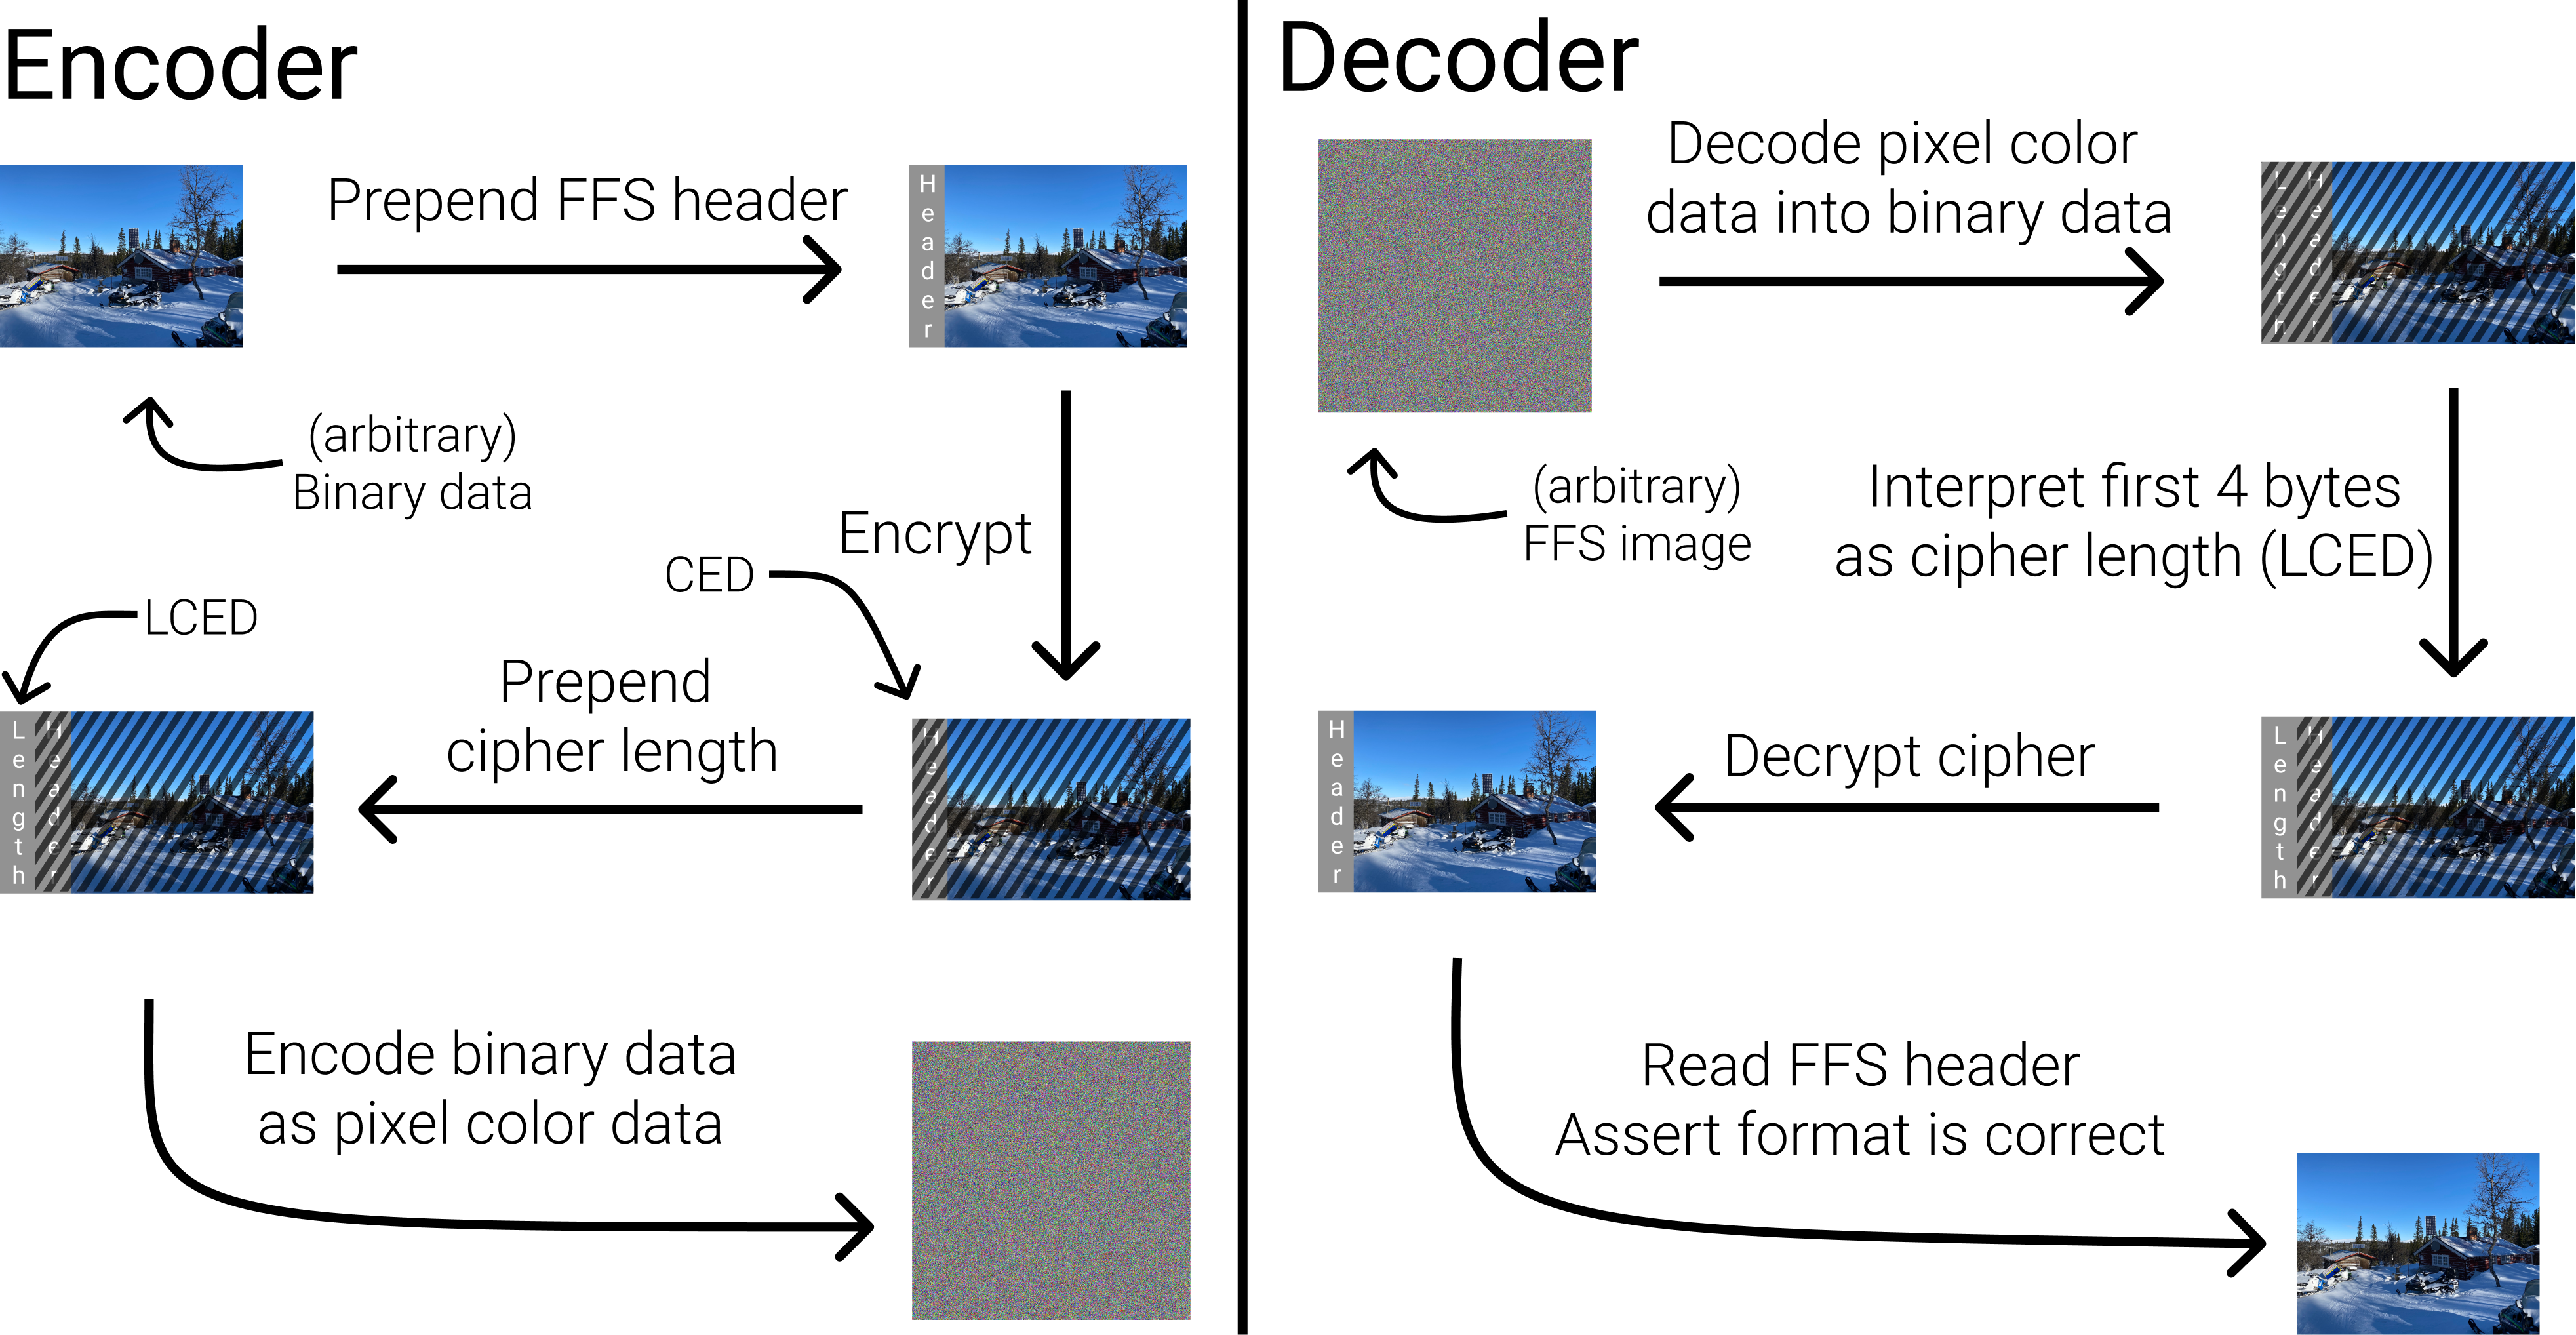
\includegraphics[width=1.0\textwidth]{figures/encoder_decoder.png}
	\end{center}
	\caption{Simple visualization of the encoder and decoder of FFS. The input of the encoder is the binary data to store in FFS, eg. a file, and the output is the FFS image to upload to the OWS. The input to the decoder is an FFS image, and the output is the binary data stored on FFS, eg. a file}
	\label{fig:file_enc_dec}
\end{figure}

\subsection{Online web services}
As FFS is a proof-of-concept filesystem, it only uses one OWS as its storage medium. However, for a production filesystem, multiple OWSs would be beneficial. This would enable features such as redundancy by using replication over multiple OWSs, for instance in case one OWS would stop working.

The initial intention of FFS was to use Twitter as the OWS. Initial research found that it was possible to upload a file and download the same file without any data loss. However, it was later found that this was not a reliable conclusion. Some images uploaded to Twitter were converted to another image format when they were stored by Twitter, which meant that the decoder could not decode the data as it expected another image format. Other images where compressed or recoded which led to data loss when downloading the image. As the decoder of FFS images relies on a specific binary representation of the image, this meant that the images could not be decoded into the previously uploaded data. 

Flickr saves the original version of the uploaded image and thus it can be used to download the same image as was uploaded. This also means that a file that is encoded into a FFS-encoded image can be uploaded, downloaded, and decoded into the same file as before. While they do not assure that they will always support original images, they also do not indicate that this would change. Therefore, Flickr can be used at this moment for the proof-of-concept filesystem that FFS is. A free-tier Flickr account is therefore used for FFS. 

% TODO: 
As mentioned in Subsection~\ref{subsec:ows_flickr}, a free-tier Flickr account can store up to 1'000 images, and each image can be up to \SI{200}{\mega\byte}. To use as few images as possible per file or directory, 

Flickr provides an extensive free REST API for non-commercial use. A user can create applications and generate access tokens for the application. These application tokens are later used to request tokens from users who authenticate using Flickr's web interface, and allow the application to do requests for the user. The application will then receive access tokens for the user, which are used to authenticate with the API for the API calls that require authentication.

As mentioned previously, Flickr provides the ability to tag an image with a number of custom tags. Every tag is a string that the user defines. By tagging the inode table with a pre-defined string we can identify the inode table easily. The Flickr API supports searching for images with a specific tag, and to filter this result by the user who uploaded the image. This allows FFS to easily find the images tagged with the pre-defined inode table tag on Flickr, uploaded by FFS. Further, ensuring that only the inode table is tagged with this tag, and by deleting the old version of the inode table on Flickr when a new version is uploaded to Flickr, we can ensure a singelton pattern of the inode table in the OWS. 

While the API is extensive in its functionality, FFS only uses a few of the provided capabilities. The Flickr API capabilites that FFS utilizes are:
\begin{itemize}
	\item Upload an image, optionally with defined tag, and return a post ID,
	\item Search for a tag of an image, uploaded by a specific user, and return the URL to the original uploaded image,
	\item Get the URL to the original uploaded image given a post ID, and
	\item Remove an image given a post ID.
\end{itemize}

To download the original image given a post ID or a tag, two requests are required:
\begin{itemize}
	\item Getting the URL to the original image using the post ID or tag,
	\item Downloading the image from the URL received from the previous request.
\end{itemize}
The second request does not require authentication as the previous request returns a public URL to the image. 

For benchmarking purposes, FFS also provides the possibility to compile the program to use a Fake OWS (FOWS), which stores the data on the local filesystem. The FOWS is used by FFS similar to how Flickr is used, by storing encoded images in it. By storing the images on the local filesystem, the filesystem operations require much lower latency than the network-based operations as FFS can avoid making requests to Flickr. This makes it easier to conclude how much of the filesystem operation time is affected by the time of the network requests. The time $T$ of a filesystem operation can be modeled like:
$$
	T = t_{ffs} + t_{ows}
$$
where $t_{ffs}$ is the time that FFS takes to, for example for a file read operation;
\begin{itemize}
	\item to find the file in the inode table,
	\item decode and decrypt the image data,
	\item read the specified amount of data, and,
	\item to output the data
\end{itemize}
This time will be approximately consistent for the same request. However, cache misses/hits and process scheduling can fluctuate the value of $t_{ffs}$. $t_{ows}$ is the total time required to complete all requests to the OWS for a filesystem operation. For instance, for a similar read operation as above;
\begin{itemize}
	\item to find the inode table given the tag,
	\item download the inode table, and,
	\item to download the images representing the file to read
\end{itemize}
Depending on the OWS, the latency and bandwidth of the internet connection between the user's machine and the OWS's server can differ a lot. Duplicate requests to the same OWS can also differ significantly due to, for instance, server load balancing and a difference in request quantity from other users at the time of the requests. However, for a FOWS, $t_{ows}$ can be replaced by $t_{fows}$ which will have approximately consistent values for duplicate operations, as the local filesystem is not affected as much by load balancing. The local filesystem requests by other applications can also be influenced and minimized by not using other applications on the machine while running the benchmarking tool to ensure filesystem requests by the FOWS can be handled quickly by the operating system. However, $t_{fows}$ is affected by, among other things, the underlying storage device of the local filesystem and process scheduling which can still fluctuate the value of $t_{fows}$.

\subsection{Implemented filesystem operations}
\label{subsec:file_op}
Following is a detailed description of all the FUSE operations implemented by FFS, and how they are implemented by FFS. Further explanations about the intended functionality of the operations can be found in \,\cite{kuenningCS135FUSEDocumentation2010}. 

The path of a file is sometimes provided for the filesystem operation and traversed by FFS to understand the requested location. An example path is \texttt{/foo/bar/buz.txt} or \texttt{/foo/bar/baz/}. A path is traversed like the following pseudo code:
\begin{lstlisting}[language=python, caption={Pseudocode of traversing a given path, returning the \texttt{Directory} and the filename}, label=lst:traverse_path,breaklines=true]
# Traverse a given path and return the parent directory object
#  and filename of the path
traverse_path(path) -> (Directory, string):
	# Fetches inode table from the OWS
	inode_table := get_inode_table()
	
	split_path := path.split("/")
	# The filename could be either the name of a file 
	#  or the name of a directory
	filename := split_path.last
	dirs := split_path.remove_last()

	# Get the root dir from cache
	curr_dir = cache.get_root_dir()

	# While there are still directories to traverse,
	#  get the next directory in the list from current
	#  directory
	while(!dirs.empty())
		dir_name := dirs.pop_first()
		inode := curr_dir.inode_of(filename=dir_name)
		inode_entry = inode_table.entry_of(inode=inode)
		# Download the image posts defined by the 
		#  post IDs in the inode entry
		curr_dir = download_as_dir(inode_entry)
	
	return (curr_dir, filename)

\end{lstlisting}

By traversing a path, FFS has to fetch all parent directories in the hierarchy. The file or directory with the filename is not fetched during while traversing the path, as it might not be necessary for the operation. This implies that all operations that relies on the path of the file or directory has to download all parent directories of the path. However, the directories in the path could be cached and therefore not require a download from the OWS. Further, \texttt{open}, \texttt{opendir}, and \texttt{create} can associate a file handle with a file or directory, so that certain other operations can use the file handle instead of traversing the string path. This saves time because the path traversing result is saved in the filesystem state.

After every operation that modifies the inode table, the inode table is uploaded to the OWS and cached. Therefore, it is assumed that the inode table is always up to date in memory and on the OWS. This will be true as long as there are not multiple FFS instances working with the same OWS account at the same time. This scenario has undefined behavior as there is no locking implemented for FFS.

All filesystem operations are synchronous unless specified. Further, FUSE is running in single-thread mode meaning that a filesystem operation call must complete before another can begin. This helps limiting the risk of data races as two processes cannot call different operations that, for instance, modify the inode table at the same time.

\subsubsection{open}
Given a path to a file, the file is associated with a file handle. The file handle is used in subsequent operations to avoid traversing the filepath. The file is not downloaded from the OWS, only the parent directories are downloaded during the path traversing as explained above. An \texttt{open} call must, eventually, be followed by a \texttt{release} call. Although, multiple other operation calls can occur between these events.

\subsubsection{release}
Given a file handle, this operation closes the file in the filesystem, disassociating the file handle with the file. The current states of the file and the inode table are saved to the OWS, and the previous versions of the file and inode table are deleted from the OWS. Subsequent operations for the file will require path traversing as the file handle can no longer be used.

The file must have a file handle associated with it before \texttt{release} is called. This requires a preceding \texttt{open} or \texttt{create} call for the file.

\subsubsection{opendir}
Given a path to a directory, the directory and associated with a file handle. The file handle is used in subsequent operations to avoid traversing the filepath. The directory is not downloaded from the OWS, only the parent directories are downloaded during the path traversing as explained above. An \texttt{opendir} call must, eventually, be followed by a \texttt{releasedir} call. Although, multiple other operation calls can occur between these events.

\subsubsection{releasedir}
Given a file handle, this operation closes the directory in the filesystem, disassociating the file handle with the directory. The current states of the directory and the inode table are saved to the OWS, and the previous versions of the directory and inode table are deleted from the OWS. Subsequent operations for the file will require path traversing as the file handle can no longer be used.

The directory must have a file handle associated with it before \texttt{releasedir} is called. This requires a preceding \texttt{opendir} call.

\subsubsection{create}
This operation creates an empty file in the filesystem given a path, and associates a file handle with the file, similar to \texttt{open}. The empty file will not be uploaded to the OWS as it has no data associated with it. A new entry is added to the parent directory with the filename and a generated inode, and the parent directory is uploaded to the OWS. The new posts representing the parent directory in the OWS is associated with the inode entry of the parent directory in the inode table, and the old posts are deleted in the OWS. An new inode entry is also created in the inode table, representing the new, empty, file.

\subsubsection{mkdir}
This operation creates an empty directory in the filesystem given a path. The directory is not uploaded to the OWS as it has no data associated with it. The parent directory is modified so it is uploaded to the OWS, and the old versions of the parent directory is deleted on the OWS. The parent directory entry in the inode table is modified with the new posts, and a new entry is created for the new directory. The inode table is updated in the OWS.

As opposed to \texttt{create} for files, this operation does not associate a file handle with the directory.

\subsubsection{read}
This operation reads a number of bytes, starting from a set offset, from the file specified by the file handle. The data is read into a provided buffer. The full file is downloaded and read into memory, even if just a small part of the file is requested. The file is also cached so that subsequential requests for the same file are faster. 

\subsubsection{readdir}
This operation reads the filenames inside the directory specified by a file handle. The result includes all filenames in the directory, and the special \texttt{"."} and \texttt{".."} directories.

\subsubsection{write}
This operation writes $s$ bytes, starting at the provided offset $o$, to the existing file at the provided file handle. All the data of the current file is read in to memory. Starting from the offset, the new data overwrites the current data of the file, until $s$ bytes have been written. If $o + s$ is greater than the file's size, the file size is set to $o + s$. If $o + s$ is less than the file's size, the data from position $o + s$ and forward remains the same, and the file size is not modified. See Figure~\ref{fig:write_flow} for a visualization. The parent directory does not have to modified. 

The file and inode table are not updated to the OWS, this occurs instead in the subsequent \texttt{release} call.

\begin{figure}[!ht]
	\begin{center}
	  
\includegraphics[width=0.9\textwidth]{figures/write_flow.png}
	\end{center}
	\caption{Visualization of how the write operation handles different offsets.}
	\label{fig:write_flow}
\end{figure}

\subsubsection{rename}
This operation renames a file or directory to a new path. Both the old path and the new path have to be traversed to located the parent directories and the file or directory to rename. The file or directory entry in the old parent directory is removed, and the old parent directory is updated to the OWS. A new entry is created in the new parent directory, with the new filename. The new parent directory is updated to the OWS. The inode entry of the renamed file or directory does not have to be modified. However, as both the old parent directories and the new parent directory are updated in the OWS, their inode entries need to be updated with the new posts. The inode table is updated to the OWS and the old table is removed from the OWS. The old posts associated with the old parent directory and the new parent directory are removed from the OWS.

The new path could be in the same directory as the file or directory currently is in. This will not affect the process mentioned above, however the path will only have to be traversed once.

\subsubsection{truncate}
This operation truncates or extends the file in the given path, to the provided size $s$ . The full current file is downloaded into memory. The data of the current file is read into a new buffer until either the file is fully read, or until $s$ bytes have been read. If the current file's size is smaller than $s$, the remaining amount of bytes are added as the NULL character. The new file data is uploaded to the OWS, and the old data is removed from the OWS. The inode table entry is updated with the new posts and uploaded to the OWS. The old inode table is removed from the OWS.

\subsubsection{ftruncate}
This operation is similar to \texttt{truncate}, but is called from a user context which means it has a file handle associated with it. The operation truncates or extends the file in the given file handle, to the provided integer $s$. The full current file is downloaded into memory. The data of the current file is read into a new buffer until either the file is fully read, or until $s$ bytes have been read. If the current file's size is smaller than $s$, the remaining amount of bytes are added as the NULL character.

The file and inode table are not updated to the OWS, this occurs instead in the subsequent \texttt{release} call.

\subsubsection{unlink}
This operation removes a file given the filepath. The file is removed from the parent directory, and the parent directory is updated to the OWS. The old parent directory data is removed on the OWS. The removed file's entry in the inode table is also removed, and the inode table updates the entry for the parent directory with its new posts. The inode table is then updated on the OWS and the old inode table is removed on the OWS. Finally, the data of the removed file is removed from the OWS. The last step is not necessary for a working filesystem; however, to save space on the OWS, this is done. If the OWS permits unlimited images and sizes, this step could be omitted to execution save time.

\subsubsection{rmdir}
Similar to \texttt{unlink}, this operation removes the directory at the path. The directory and all its subdirectories are traversed, and the post IDs of these files and directories are recorded for deletion in the OWS later. Following, the entry of the removed directory is removed from the parent directory. The inode entry for the removed directory is removed. The parent directory is updated to the OWS, and the inode table is updated with the new posts of the parent directory. Following, the inode table is updated to the OWS. The old parent directory and the old inode table are removed from the OWS.

The operation also starts a new thread, where all the posts of files and subdirectories inside the removed directory, are removed from the OWS. This occurs to save space on the OWS, and a separate thread is used to save computation time for subsequent file operations. There is no data race involved as the API is thread safe, and the posts are no longer associated with any data structures on the main thread.

\subsubsection{getattr}
This operations returns attributes about a file or directory given a path. This includes permissions, number of entries (if the provided path points to a directory), and timestamps of creation, last access and last modification. However, as mentioned previously, FFS does not implement all features, such as permissions. Instead of keeping track of a file's or directory's permissions, all calls to valid path will return full read, write, and execute permissions for everyone. However, the timestamps are stored in the inode table of FFS. The file or directory pointed to by the path does not need to be downloaded, all the metadata that FFS stores is accessible through the inode entry in the inode table.

\subsubsection{fgetattr}
This operation is the similar to \texttt{getattr}, but is called from a user program context meaning that the file has a file handle associated with it. Other than skipping the path traverse step, this operation returns the equivalent information as \texttt{getattr}.

\subsubsection{statfs}
This operation returns metadata information about FFS. This includes, among other things, the maximum filename size and the filesystem ID. The operation has a short computation time as it does not have to download or upload any files. The only variable information is read from the inode table which is stored in memory and thus does not have to be downloaded from the OWS.

\subsubsection{access}
This operation, given a path, returns wether or not the path can be accessed. As long as the path is valid, this always returns that it can be accessed.

\subsubsection{utimens}
This operation updates the last access timestamp, the last modified timestamp, or both, of the file or directory at the given path. The file or directory does not have to be downloaded. However, the inode entry for the file's or directory's inode is updated with the new timestamps if they are newer than the previous timestamps but not greater than the current time since epoch. The new state of the inode table is updated to the OWS, and the old version is removed from the OWS.

% \subsection{Unimplemented filesystem operations}
% FIXME: Is this needed? ^ 

\subsection{FFS limitations}
% TODO: Limitations, both in number of bytes, files etc
% Also what it lacks, such as filesystem operations and speed(!)
FFS has numerous of limitations due to both implementation decisions and OWS limits. As Flickr allows a free-tier user account to store up to 1\,000 images of up to \SI{200}{\mega\byte} per image, this allows storage of up to \SI{200}{\giga\byte} of images on per account on Flickr. However, as the inode table is required to be stored on the filesystem, a maximum of 999 images can be used to save file and directory data. This limits the filesystem to a maximum of 999 files and directories while utilizing one free-tier account on Flickr. 

While Flicker supports each image to be up to \SI{200}{\mega\byte}, it is not possible to use the full \SI{200}{\mega\byte} as the file data to store. The image includes, among other things, a PNG header, and the data stored is encrypted which could result in a cipher text of greater size than the unencrypted data.

This gives the system a maximum storage capacity of \SI{199.6}{\gia\byte} of FFS images. However, this assumes that all images are at their max capacity. As each file with data requires at least one image, there can be a maximum of 998 files and directories in the filesystem, excluding the root directory. 

FFS limits the directories and the inode table to only occupy one image each. 

FFS:
200MB per photo, 1000 photos for free == 200GB of maximum storage
Using videos of 1GB per, could get up to 1TB of maximum storage
Multiple accounts could expand this further

Limited on bandwidth